\section{Стохастический анализ}

    \subsection{Описание изменений}

        После завершения детерминированного анализа можно перейти к стохастическому анализу. В модели (\ref{origin}) появляется слагаемое, которое отвечает за шум. Это слагаемое имеет следующий вид: \(\varepsilon \xi\), где \(\varepsilon\) --- интенсивность шума, а \(\xi\) --- нормальная случайная величина.

        Каждый вид шума несет свой биологический смысл. Например, увеличение численности популяции может происходить неравномерно из-за внешних обстоятельств, такому поведению системы соответствует \(\alpha\)-шум. \(\beta\)-шум показывает, что среда обитания также может в зависимости от времени предоставлять разное количество ресурсов для поддержания численности популяции. И наконец, аддитивный шум показывает, что рассматриваемая среда обитания необязательно должна быть изолирована от окружающего мира, поэтому будет наблюдаться миграция особей.

        \comment{А что насчет комбинации шумов? Какие-то события могут влиять на enviroment capacity и на growth rate одновременно. Еще сложнее анализировать. Сложнее проанализировать.}

        Вот так будут выглядеть формулы с разными видами шума.

        \(\alpha\)-шум: 

        \begin{equation}
            \label{alpha_chaos}
            x_{t + 1} = \frac{(\alpha + \varepsilon \xi) x_t^2}{(\beta + x_t)^6}
        \end{equation}

        \(\beta\)-шум:

        \begin{equation}
            \label{beta_chaos}
            x_{t + 1} = \frac{\alpha x_t^2}{(\beta + \varepsilon \xi + x_t)^6}
        \end{equation}

        Аддитивный шум:

        \begin{equation}
            \label{additive_chaos}
            x_{t + 1} = \frac{\alpha x_t^2}{(\beta + x_t)^6} + \varepsilon \xi
        \end{equation}

    \subsection{Временные ряды}

        С помощью временных рядов продемонстрируем как различные виды шума влияют на поведение системы. Рассмотрим сразу все возможные виды шума. 

        На рисунке \ref{time_series_x_0_06_a_1_b_0_56} изображено поведение модели без добавления каких-либо шумов. Мы видим, что значения с течением времени стабилизируются. Численность популяции фактически остается неизменной на протяжении всего длительного времени.

        \begin{figure}
            \centering
            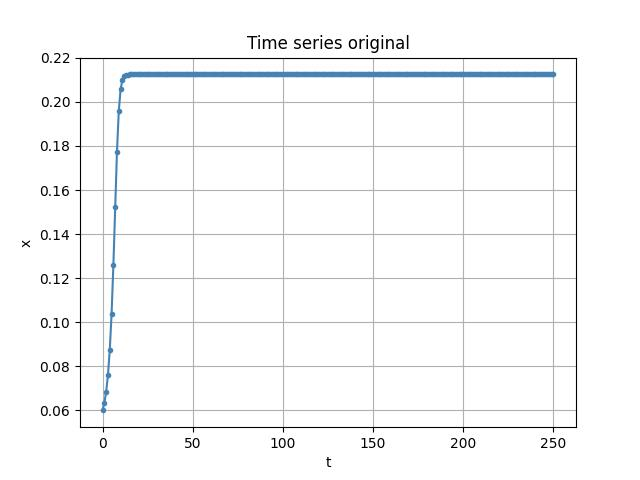
\includegraphics[width=\textwidth]{stochastic/time_series_x_0_06_a_1_b_0_56.jpg}

            \captionsetup{justification=centering}
            \caption{Временной ряд модели (\ref{origin}) при \(\beta = 0.56, \alpha = 1, x_0 = 0.06\)}
            \label{time_series_x_0_06_a_1_b_0_56}
        \end{figure}

        Теперь давайте добавим шумы в нашу модель и рассмотрим соответственно рисунки \ref{time_series_x_0_06_a_1_b_0_56_alpha_chaos_epsilon_0_004}, \ref{time_series_x_0_06_a_1_b_0_56_beta_chaos_epsilon_0_004} и \ref{time_series_x_0_06_a_1_b_0_56_additive_chaos_epsilon_0_004}. Все варианты рассматриваются с одной и той же интенсивностью шума \(\varepsilon = 0.004\). 
        
        Мы видим, что вид шума влияет на величину разброса значений численности популяции. \comment{Приплети сюда дисперсию.} И если раньше численность популяции стабилизировалась и переставала хоть сколько-нибудь меняться, то сейчас численность постоянно всегда колеблется, но как можно заметить, она меняется в рамках некоторого коридора значений. Численность популяции в общем то не растет и не уменьшается на какую-то значительную величину. Но такое поведение наблюдается не всегда.

        \comment{малый шум будет оказывать незначительное влияние, а большой - огромное.}

        \comment{Можно взять оригинальный временной ряд и на него сверху наложить временной ряд с шумом.}

        \comment{Хорошая фраза: переход вызванный индуцированным шумом}

        \begin{figure}
            \centering
            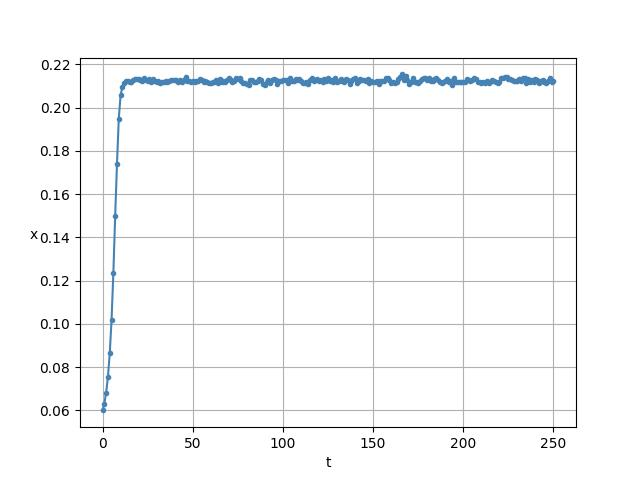
\includegraphics[width=\textwidth]{stochastic/time_series_x_0_06_a_1_b_0_56_alpha_chaos_epsilon_0_004.jpg}
        
            \captionsetup{justification=centering}
            \caption{Временной ряд модели (\ref{alpha_chaos}) при \(\beta = 0.56, \alpha = 1, x_0 = 0.06, \varepsilon = 0.004\)}
            \label{time_series_x_0_06_a_1_b_0_56_alpha_chaos_epsilon_0_004}
        \end{figure}

        \begin{figure}
            \centering
            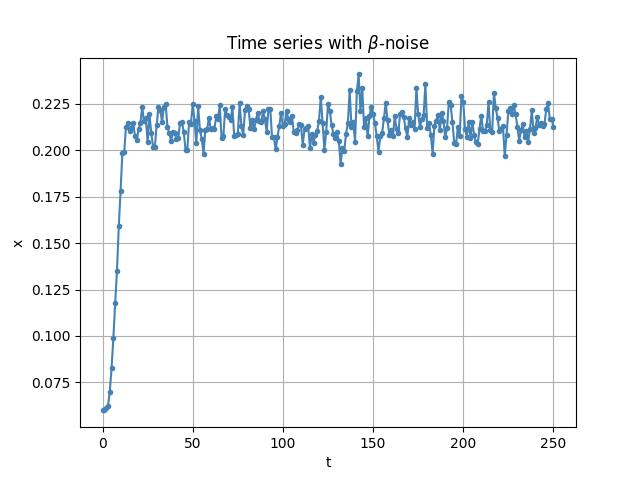
\includegraphics[width=\textwidth]{stochastic/time_series_x_0_06_a_1_b_0_56_beta_chaos_epsilon_0_004.jpg}
        
            \captionsetup{justification=centering}
            \caption{Временной ряд модели (\ref{beta_chaos}) при \(\beta = 0.56, \alpha = 1, x_0 = 0.06, \varepsilon = 0.004\)}
            \label{time_series_x_0_06_a_1_b_0_56_beta_chaos_epsilon_0_004}
        \end{figure}

        \begin{figure}
            \centering
            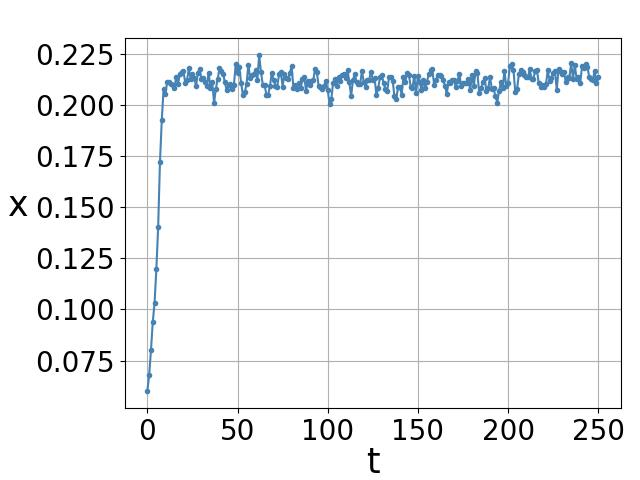
\includegraphics[width=\textwidth]{stochastic/time_series_x_0_06_a_1_b_0_56_additive_chaos_epsilon_0_004.jpg}
        
            \captionsetup{justification=centering}
            \caption{Временной ряд модели (\ref{additive_chaos}) при \(\beta = 0.56, \alpha = 1, x_0 = 0.06, \varepsilon = 0.004\)}
            \label{time_series_x_0_06_a_1_b_0_56_additive_chaos_epsilon_0_004}
        \end{figure}

        Для того чтоб продемонстрировать другое возможное поведение, давайте увеличим интенсивность шума. Пускай теперь \(\varepsilon = 0.04\). Рассмотрим рисунок \ref{time_series_x_0_06_a_1_b_0_56_beta_chaos_epsilon_0_04_fall}. Здесь мы видим ситуацию, когда шум оказал негативное влияние на численность популяции. Но опять же все не так просто. Если мы еще раз запустим алгоритм, который просчитывает нашу модель, то мы увидим, что популяция успешно выживала на протяжении анализируемого интервала времени. Данный пример проиллюстрирован на картинке \ref{time_series_x_0_06_a_1_b_0_56_beta_chaos_epsilon_0_04_alive}. Аналогичные эффекты можно наблюдать и при других видах шума.

        \comment{Примерно в \(t = 50\) обе популяции были близки к вымиранию, но одна выжила, а вторая нет. "Одно рисовое зернышко может склонить чашу весов" (с) какой-то мультик.}

        \begin{figure}
            \centering
            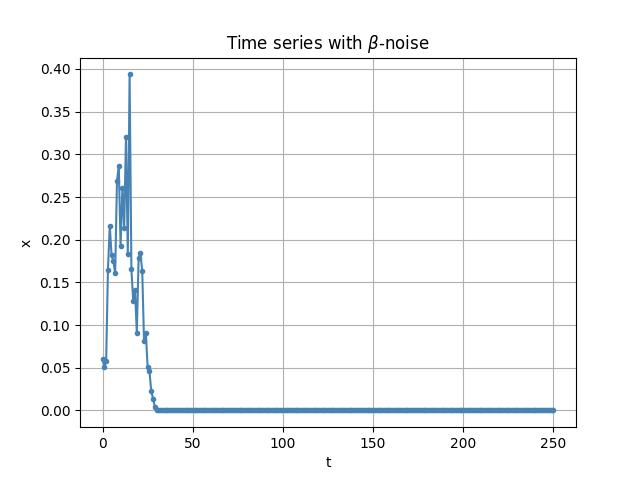
\includegraphics[width=\textwidth]{stochastic/time_series_x_0_06_a_1_b_0_56_beta_chaos_epsilon_0_04_fall.jpg}
        
            \captionsetup{justification=centering}
            \caption{Временной ряд модели (\ref{beta_chaos}) при \(\beta = 0.56, \alpha = 1, x_0 = 0.06, \varepsilon = 0.04\)}
            \label{time_series_x_0_06_a_1_b_0_56_beta_chaos_epsilon_0_04_fall}
        \end{figure}

        \begin{figure}
            \centering
            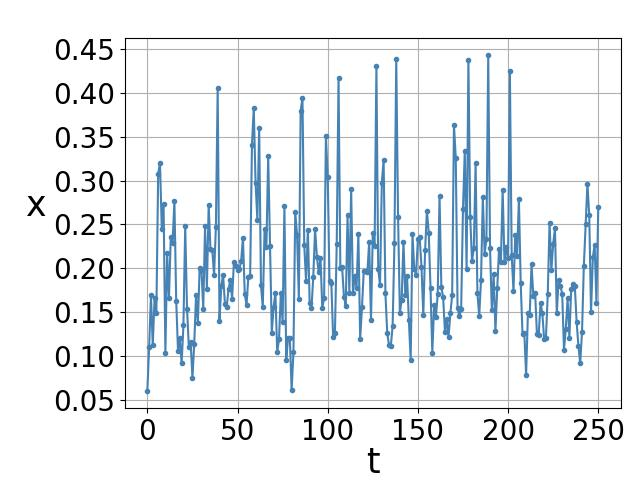
\includegraphics[width=\textwidth]{stochastic/time_series_x_0_06_a_1_b_0_56_beta_chaos_epsilon_0_04_alive.jpg}
        
            \captionsetup{justification=centering}
            \caption{Временной ряд модели (\ref{beta_chaos}) при \(\beta = 0.56, \alpha = 1, x_0 = 0.06, \varepsilon = 0.04\)}
            \label{time_series_x_0_06_a_1_b_0_56_beta_chaos_epsilon_0_04_alive}
        \end{figure}

        Анализируя вышесказанное можно сказать, что при добавлении в модель случайных событий ее поведение становится непредсказуемым. Одно незначительное изменение может кардинально повлиять на ход развития событий. 

        \comment{рассматривать как в том семестре все возможные варианты поведения системы в зависимости от начальной точки думаю не надо и так все понятно.}

    \subsection{Бифуркация}

        Теперь перейдем к рассмотрению графиков бифуркации с разными видами шумов. Все то же самое, только картинка не такая четкая.

        \begin{figure}
            \centering
            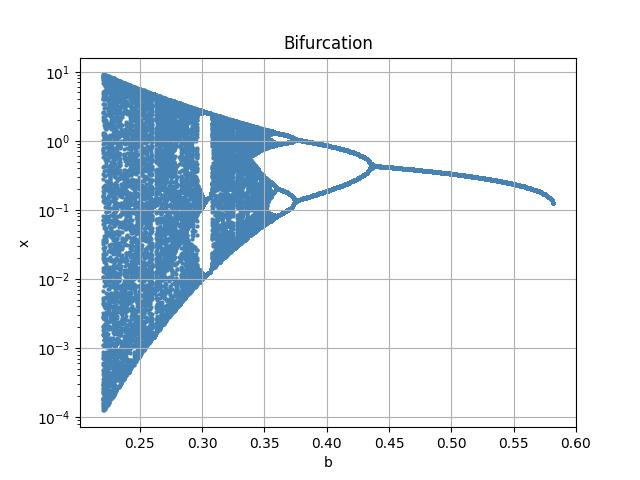
\includegraphics[width=\textwidth]{stochastic/bifurcation_x_0_2_a_1_compare_no_noise.jpg}
        
            \captionsetup{justification=centering}
            \caption{График бифуркации без шума}
            \label{bifurcation_x_0_2_a_1_compare_no_noise}
        \end{figure}

        \begin{figure}
            \centering
            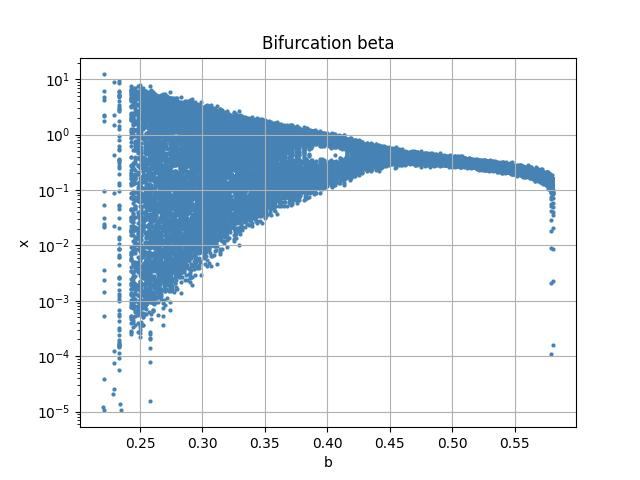
\includegraphics[width=\textwidth]{stochastic/bifurcation_x_0_2_a_1_compare_beta_noise.jpg}
        
            \captionsetup{justification=centering}
            \caption{График бифуркации с \(\beta\)-шумом, \(\varepsilon = 0.01\)}
            \label{bifurcation_x_0_2_a_1_compare_beta_noise}
        \end{figure}

        \begin{figure}
            \centering
            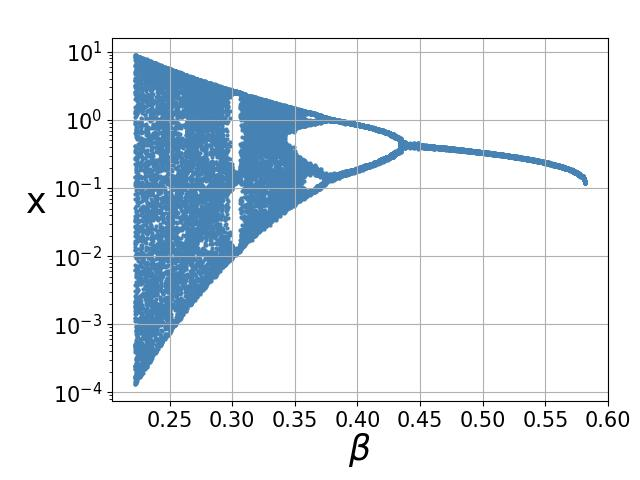
\includegraphics[width=\textwidth]{stochastic/bifurcation_x_0_2_a_1_compare_alpha_noise.jpg}
        
            \captionsetup{justification=centering}
            \caption{График бифуркации с \(\alpha\)-шумом, \(\varepsilon = 0.01\)}
            \label{bifurcation_x_0_2_a_1_compare_alpha_noise}
        \end{figure}

        \begin{figure}
            \centering
            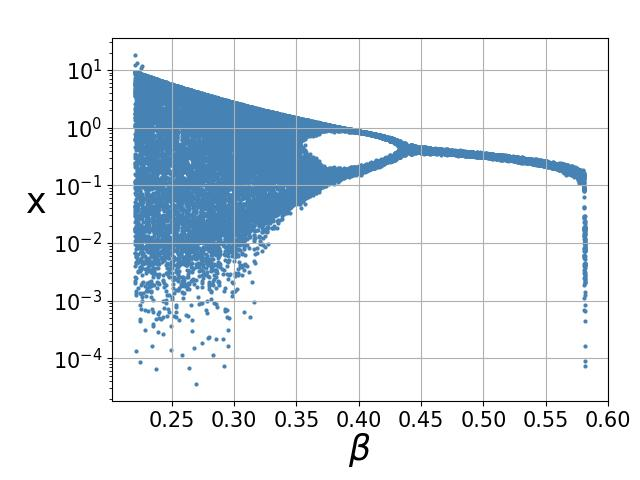
\includegraphics[width=\textwidth]{stochastic/bifurcation_x_0_2_a_1_compare_additional_noise.jpg}
        
            \captionsetup{justification=centering}
            \caption{График бифуркации с аддитивным шумом, \(\varepsilon - 0.01\)}
            \label{bifurcation_x_0_2_a_1_compare_additional_noise}
        \end{figure}

        \comment{напиши что-нибудь про бифуркацию}

    \subsection{Матожидание}

        \comment{напиши что-нибудь про матожидание и циклическое матожидание}

    \subsection{Дисперсия}

        \comment{напиши что-нибудь про дисперсию и циклическую дисперсию}

    \subsection{Функция стохастический чувствительности}
    
        Функция стохастический чувствительности это инструмент, который показывает... 

        \comment{Думаю формулы тут не нужны, оставить ссылку на статью Crises, noise, and tipping in the Hassell population model}

        Давайте посмотрим на график \ref{bifurcation_x_0_2_a_1_beta_chaos_fss}. Красными линиями нарисована функция стохастический чувствительности. \comment{напиши зачем она тут вообще нужна}. 

        \begin{figure}
            \centering
            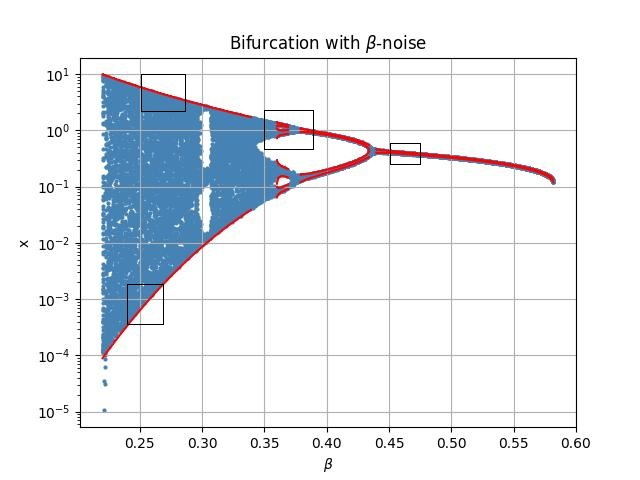
\includegraphics[width=\textwidth]{stochastic/bifurcation_x_0_2_a_1_beta_noise_fss.jpg}
        
            \captionsetup{justification=centering}
            \caption{График бифуркации с \(\beta\)-шумом.}
            \label{bifurcation_x_0_2_a_1_beta_chaos_fss}
        \end{figure}

        Рассмотрим участок от \(\beta \approx 0.45\) до \(\beta \approx 0.48\), он изображен на рисунке \ref{bifurcation_x_0_2_a_1_beta_chaos_fss_segment_stable}. Мы видим, что значения графика бифуркации почти всегда находятся в коридоре, границами которого являются значения ФСЧ. Этот коридор строится по правилу трех сигм. Такой подход гарантирует, что почти все значения будут находиться в этом интервале, что собственно мы и наблюдаем.

        \begin{figure}
            \centering
            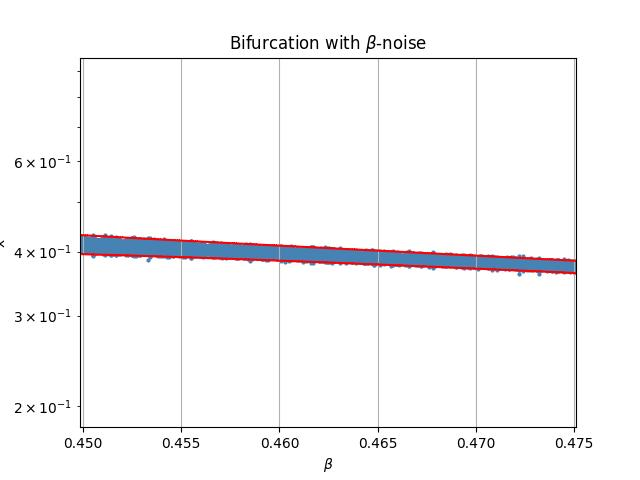
\includegraphics[width=\textwidth]{stochastic/bifurcation_x_0_2_a_1_beta_noise_fss_segment_stable.jpg}
        
            \captionsetup{justification=centering}
            \caption{}
            \label{bifurcation_x_0_2_a_1_beta_chaos_fss_segment_stable}
        \end{figure}

        На участках с k-циклами и хаосом (рисунки \ref{bifurcation_x_0_2_a_1_beta_chaos_fss_segment_2_cycle}, \ref{bifurcation_x_0_2_a_1_beta_chaos_fss_segment_chaos_up} и \ref{bifurcation_x_0_2_a_1_beta_chaos_fss_segment_chaos_down]}) будет наблюдаться аналогичная ситуация: значения лежат в коридоре, ограниченном значениями ФСЧ.

        \begin{figure}
            \centering
            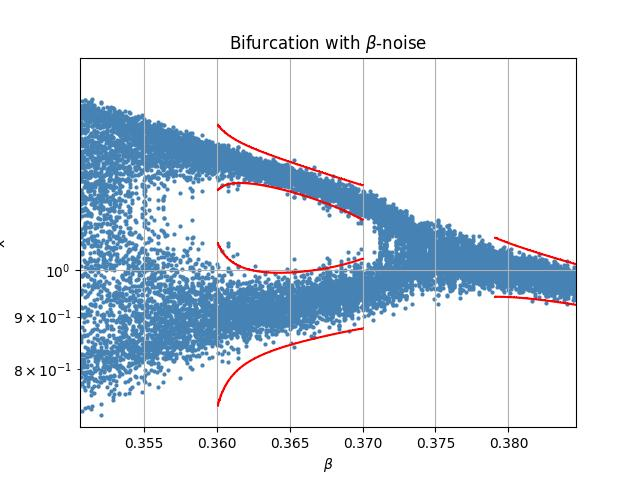
\includegraphics[width=\textwidth]{stochastic/bifurcation_x_0_2_a_1_beta_noise_fss_segment_2_cycle.jpg}
        
            \captionsetup{justification=centering}
            \caption{}
            \label{bifurcation_x_0_2_a_1_beta_chaos_fss_segment_2_cycle}
        \end{figure}

        \begin{figure}
            \centering
            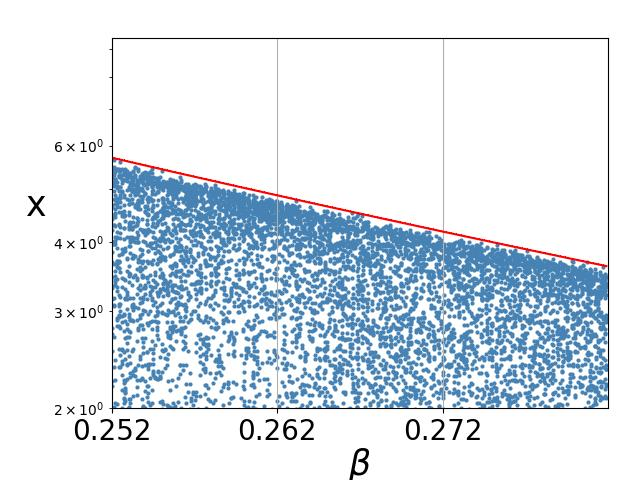
\includegraphics[width=\textwidth]{stochastic/bifurcation_x_0_2_a_1_beta_noise_fss_segment_chaos_up.jpg}
        
            \captionsetup{justification=centering}
            \caption{}
            \label{bifurcation_x_0_2_a_1_beta_chaos_fss_segment_chaos_up}
        \end{figure}

        \begin{figure}
            \centering
            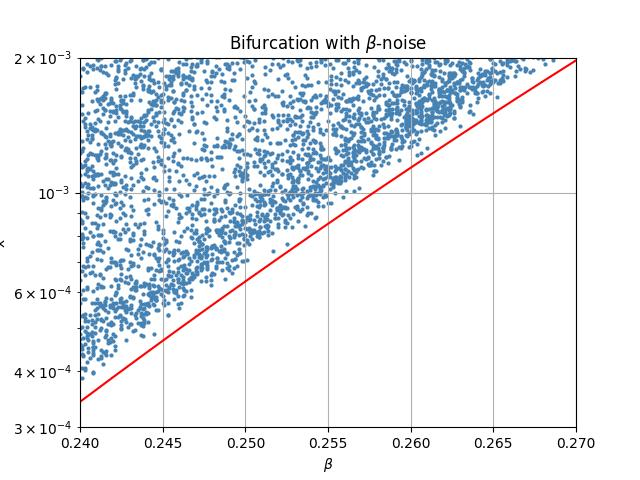
\includegraphics[width=\textwidth]{stochastic/bifurcation_x_0_2_a_1_beta_noise_fss_segment_chaos_down.jpg}
        
            \captionsetup{justification=centering}
            \caption{}
            \label{bifurcation_x_0_2_a_1_beta_chaos_fss_segment_chaos_down}
        \end{figure}

        \comment{напиши что-нибудь про ФСЧ}

    \subsection{График ФСЧ}

        \comment{напиши что-нибудь про график фсч, это который m(beta)}

    \subsection{Критическая интенсивность}

        Критическая интенсивность --- значение интенсивности, при которой траектории могут выходить за границы аттрактора и сваливаться в ноль.

        Например, на рисунке \ref{critical_intensity_beta_noise} изображен график Критической интенсивности для \(\beta\)-шума.

        \comment{Просчитай эти графики для более мелкого шага, чтоб точки были ближе друг к другу}

        \begin{figure}
            \centering
            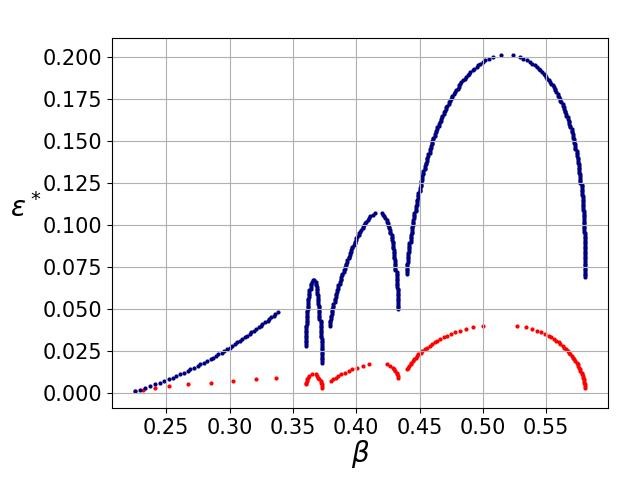
\includegraphics[width=\textwidth]{stochastic/critical_intensity_beta_noise.jpg}
        
            \captionsetup{justification=centering}
            \caption{}
            \label{critical_intensity_beta_noise}
        \end{figure}
        